\documentclass[]{article}
\usepackage[UTF8]{ctex}
\usepackage{amsmath}
\usepackage{xcolor}
\usepackage{tikz}
\usetikzlibrary{positioning} %为了实现相对位置的设定
\usepackage{xcolor} %为了实现不同的颜色
\usepackage{tikz}
\usetikzlibrary{arrows.meta}
\usepackage{tikz-network}
\usepackage{pgffor}%可以使用foreach的包
\usepackage{ifthen}%可以使用ifthenelse的包,还能使用whiledo
\usepackage{algorithm}
\usepackage{algorithmic}
\renewcommand{\algorithmicrequire}{ \textbf{Input:}} %Use Input in the format of Algorithm
\renewcommand{\algorithmicensure}{ \textbf{Output:}} %UseOutput in the format of Algorithm\usepackage{algorithm}
\usepackage{algorithmic}
\renewcommand{\algorithmicrequire}{ \textbf{Input:}} %Use Input in the format of Algorithm
\renewcommand{\algorithmicensure}{ \textbf{Output:}} %UseOutput in the format of Algorithm
%opening
\title{隐马尔科夫模型}
\author{覃一发}

\begin{document}

\maketitle

\begin{abstract}
    隐马尔科夫模型描述由隐藏的马尔科夫链随机生成观测序列的过程,属于生成模型,是可用于标注问题的统计学习模型。本章依次介绍其基本概念和要素,常见的三大任务-概率计算、学习、预测以及对应算法。隐马尔科夫模型广泛引用与语音识别、模式识别、自然语言处理、生物信息学等领域。
\end{abstract}

\section{从红蓝球盒子开始}
    假设由3个盒子,每个盒子里有红、蓝两种颜色的球,数量由下表给出。
    \begin{table}[!h]
    	\begin{center}
    		\caption{各盒子的红、蓝球数量}
    		\begin{tabular}{l|ccc}
    			\hline
    			\quad & \textbf{Box 1} & \textbf{Box 2} & \textbf{Box 3}\\
    			\hline
    			\textcolor{red}{Red} & 2 & 3 & 5 \\
    			\hline
    			\textcolor{blue}{Blue} & 4 & 3 & 1 \\
    			\hline
    		\end{tabular}	
    	\end{center}
	\end{table}
    
    按照以下的方法抽球。
    \begin{enumerate}
    	\item 从3个盒子里以等概率随机选取1个盒子,从该盒子随机抽取1个球,记录颜色后放回; 
    	\item 从当前盒子随机转移到下一个盒子,转移规则是从盒子1到盒子2概率为1,盒子2转移到盒子1概率为0.4, 到盒子3为0.6,盒子3停留自身或转移到盒子2概率都是0.5;
    	\item 确定转移的盒子后,记录颜色并放回;
    	\item 如此重复5次得到颜色的观测序列。
    	\begin{equation}
    		O=(\textcolor{red}{Red},\textcolor{red}{Red},\textcolor{blue}{Blue},\textcolor{red}{Red},\textcolor{blue}{Blue})
    	\end{equation}
    \end{enumerate}
 


    对应的盒子序列是$S=(box 1, box 2, box 3, box 3, box 2)$。
    
    上述的抽球玩法正是隐马尔科夫模型的一个简单例子,其中包含如下3个重要元素。
    
    初始3个盒子被抽中的概率$\pi$。
    \begin{equation}
    	\pi=(\frac{1}{3},\frac{1}{3},\frac{1}{3})
    \end{equation}
    
    盒子转移的概率分布$A$。$A_{ij}$ 表示从盒子i转移到盒子j的概率大小。   
    \begin{equation}
    	A = 
    	\begin{bmatrix}
    		0 & 1 & 0 \\
    		0.4 & 0 & 0.6 \\
    		0 & 0.5 & 0.5 
        \end{bmatrix}
    \end{equation}

   盒子序号和观测到的颜色的对应概率$B$。$B_{ij}$ 表示从盒子i中抽到红色(j=0)、蓝色(j=1)的概率大小。   
    \begin{equation}
   		B = 
   		\begin{bmatrix}
   			\frac{1}{3} & \frac{2}{3} \\
   			\frac{1}{2} & \frac{1}{2}  \\
   			\frac{1}{6} & \frac{5}{6} 
   		\end{bmatrix}
   \end{equation}

\section{隐马尔科夫基本概念}
    隐马尔可夫(Hidden Markov Model, 以下简称HMM)中有状态和观测。状态根据马尔科夫链在各状态间切换,形成隐藏状态序列。观测随状态更新而更新,出现概率与状态有关,形成观测序列。如下图所示。
    
    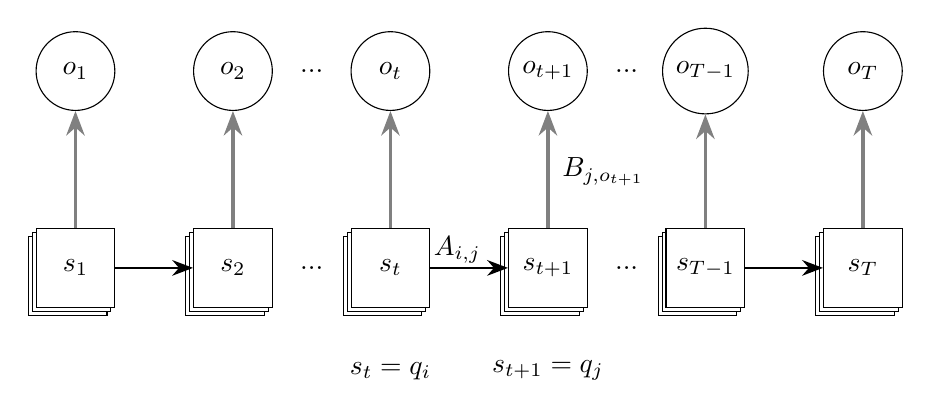
\begin{tikzpicture}[>=Stealth] % 后向算法图示
    	\foreach \i/\name in {1/$o_1$,2/$o_2$,3/$o_t$,4/$o_{t+1}$,5/$o_{T-1}$,6/$o_{T}$}{
    		\node[circle,draw,text=black,font={\bfseries},minimum size=1cm] 
    		(o\i) at (2.0*\i-2.0,2.5){\name};
    	}
    	
    	\foreach \i/\name in {1/$s_1$,2/$s_2$,3/$s_t$,4/$s_{t+1}$,5/$s_{T-1}$,6/$s_{T}$}{
    		\node[rectangle,draw,fill=white,text=black,font={\bfseries},minimum size=1cm] 
    		(sss\i) at (2.0*\i-2.0-0.1,-0.1){\name};
    		\node[rectangle,draw,fill=white,text=black,font={\bfseries},minimum size=1cm] 
    		(ss\i) at (2.0*\i-2.0-0.05,-0.05){\name};
    		\node[rectangle,draw,fill=white,text=black,font={\bfseries},minimum size=1cm] 
    		(s\i) at (2.0*\i-2.0,0){\name};
    	}
    	
    	\foreach \i in {1,2,3,4,5,6}{
    		\draw[->,color=gray,line width=1.3pt]--(s\i)--(o\i);}
    	
    	\node[](s0) at (0, 0){};
    	%	\draw[->,line width=1pt]--(s0)--(s1);
    	\draw[->,line width=1pt]--(s1)--(s2);
    	\draw[->,line width=1pt]--(s3)--(s4);
    	\draw[->,line width=1pt]--(s5)--(s6);
    	
    	%	\node[text = black,scale = 1] at ([shift=(165:20pt)] s1.center) {$\pi(s_{1})$};
    	\node[text = black,scale = 1] at ([shift=(60:40pt)] s4.center) {$B_{j,o_{t+1}}$};
    	\node[text = black,scale = 1] at ([shift=(15:25pt)] s3.center) {$A_{i,j}$};
    	
    	\foreach \i in {o2,o4, s2, s4}{
    		\node[,text = black,scale = 1] 
    		at ([shift=(0:10mm)] \i.center) {...}; } % 省略号	
    	
    	\node[,text = black,scale = 1] 
    	at ([shift=(270:8mm)] s3.south) {$s_{t}=q_{i}$}; % 省略号
    	
    	\node[,text = black,scale = 1] 
    	at ([shift=(270:8mm)] s4.south) {$s_{t+1}=q_{j}$}; % 省略号
    	
    	\label{fig.backward.algo}
    \end{tikzpicture}
    
    
    
    描述HMM(一阶)需要三大要素,分别是初始状态的概率分布向量,状态转换的概率方阵,从状态对应各观测的概率矩阵,分别记为$\pi$, $A$, $B$,如Eq.\ref{eq.hmm}。

    \begin{equation}
    	h=(\pi, A, B) \label{eq.hmm}
    \end{equation}

   $\pi_{i}$是初始时刻状态为$q_{i}$的概率;$A_{ij}$是从状态$q_{i}$转移到$q_{j}$的概率;$B_{ij}$是状态$q_{i}$呈现为第j种观测相$v_{j}$的概率。状态的集合记为$Q$,观测的集合记为$V$,$M$,$N$分别是所有可能的观测、状态数量。
   
   \begin{equation}
   		Q=\{q_{1},q_{2},...,q_{N}\},   	V=\{v_{1},v_{2},...,v_{M}\}
   \end{equation}

   	长度为T的状态序列记为S,观测序列记为O。
   \begin{equation}
		S=(s_{1},s_{2},...,s_{T}),   	O=(o_{1},o_{2},...,o_{T})
   \end{equation}
    很自然地$s_{i}\in{Q},i=1,2,...,T$;$o_{i} \in V, i=1, 2, ..., T$。
    
\section{隐马尔科夫模型的三个基本任务}    
    HMM有3个基本问题,费别是观测序列的概率计算、HMM参数估计、状态序列的预测解码问题。
    
    \begin{itemize}
    	\item \textcolor{blue}{概率计算}。 \\已知$h=(\pi, A, B)$,求特定观测序列$O$出现的概率$P(O|h)$。
    	\item  \textcolor{blue}{参数估计}。 \\已知观测序列$O$,求$h=(\pi, A, B)$使得概率$P(O|h)$最大化。
    	\item  \textcolor{blue}{预测解码}。 \\已知观测序列$O$以及$h=(\pi, A, B)$,求状态序列使得$P(S|h,O)$最大化。
    \end{itemize}

\subsection{观测序列的概率计算}
 \subsubsection{前向算法}
    我们计算的目标是观测序列$O=(o_{1}, o_{2}, ..., o_{T})$出现的概率$P(O|h)$。由于在概率计算任务里模型参数$h$已固定,为了方便后文的$P(O|h)$都改写为$P(O)$。
    
    每个时刻都对应多种可能的隐藏状态,即序列包含了隐变量$s_{t},t=1,...,T$,见图\ref{fig.forward.algo}。为了简单起见,我们只选取1个隐变量,利用边际概率公式把$P(O)$对隐变量展开,见公式\ref{eq.PO.forward}。前向算法选取的隐变量是最后的节点状态$s_{T}$。每个时刻的状态$s_{t}$都属于集合$Q=\{q_{1},q_{2},...,q_{M}\}$。
    %$P(O)=\sum_{i=1}^{N}P(O,s_{T}=q_{i})$。
    
    \begin{equation}
    	P(O)=\sum_{i=1}^{N}P(o_{1},o_{2},...,o_{T},s_{T}=q_{i}) \label{eq.PO.forward}
    \end{equation} 
    
    为了描述方便,我们定义$\alpha_{t}(i)$,见公式\ref{eq.alpha.t}。
    
    \begin{equation}
  		\alpha_{t}(i)=P(o_{1}, o_{2}, ..., o_{t}, s_{t}=q_{i}) \label{eq.alpha.t}
    \end{equation}
    
    那么观测序列的概率即可表示为$\alpha_{T}(i)$之和。
    \begin{equation}
    	P(O)=\sum_{i=1}^{N}\alpha_{T}(i) \label{eq.PO.alphaT}
    \end{equation}
    
    如图\ref{fig.forward.algo}所示。

% 前向算法图示
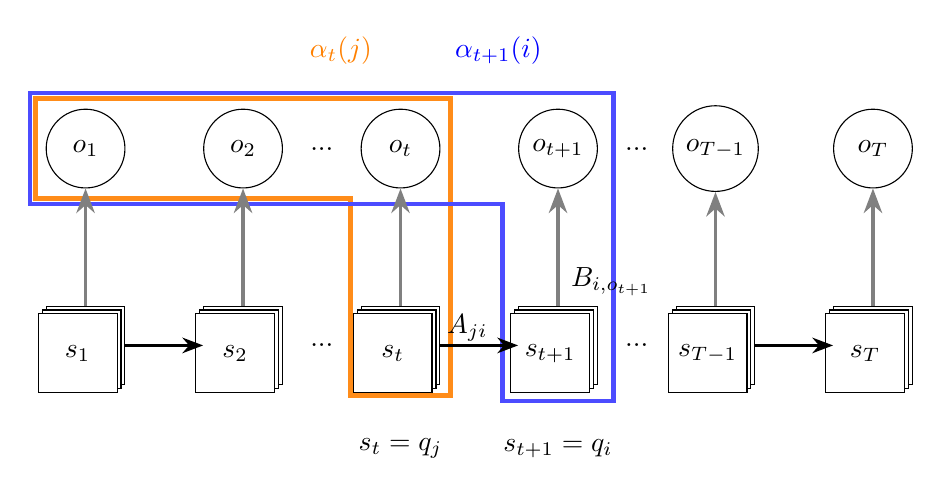
\begin{tikzpicture}[>=Stealth]
	\foreach \i/\name in {1/$o_1$,2/$o_2$,3/$o_t$,4/$o_{t+1}$,5/$o_{T-1}$,6/$o_{T}$}{
		\node[circle,draw,text=black,font={\bfseries},minimum size=1cm] 
		(o\i) at (2.0*\i-2.0,2.5){\name};
	}
	
	\foreach \i/\name in {1/$s_1$,2/$s_2$,3/$s_t$,4/$s_{t+1}$,5/$s_{T-1}$,6/$s_{T}$}{
		\node[rectangle,draw,fill=white,text=black,font={\bfseries},minimum size=1cm] 
		(s\i) at (2.0*\i-2.0,0){\name};
		\node[rectangle,draw,fill=white,text=black,font={\bfseries},minimum size=1cm] 
		(ss\i) at (2.0*\i-2.0-0.05,-0.05){\name};
		\node[rectangle,draw,fill=white,text=black,font={\bfseries},minimum size=1cm] 
		(sss\i) at (2.0*\i-2.0-0.1,-0.1){\name};
	}
	
	\draw[outer sep=0.3cm, color=orange!90,line width=1.6pt] ([shift=(135:9mm)] o1.center)--([shift=(45:9mm)] o3.center)--([shift=(315:9mm)]s3.center)--([shift=(225:9mm)] s3.center)--([shift=(225:9mm)] o3.center)--([shift=(225:9mm)]o1.center)--cycle;
	
	\draw[outer sep=0.3cm, color=blue!70,line width=1.6pt] ([shift=(135:1cm)] o1.center)--([shift=(45:1cm)] o4.center)--([shift=(315:1cm)]s4.center)--([shift=(225:1cm)] s4.center)--([shift=(225:1cm)] o4.center)--([shift=(225:1cm)]o1.center)--cycle;
	
	\foreach \i in {1,2,3,4,5,6}{
		\draw[->,color=gray,line width=1.3pt]--(s\i)--(o\i);}
	
	\node[](s0) at (0, 0){};
%	\draw[->,line width=1pt]--(s0)--(s1);
	\draw[->,line width=1pt]--(s1)--(s2);
	\draw[->,line width=1pt]--(s3)--(s4);
	\draw[->,line width=1pt]--(s5)--(s6);
	
%	\node[text = black,scale = 1] at ([shift=(15:20pt)] s0.center) {$\pi(s_{1})$};
	\node[text = black,scale = 1] at ([shift=(50:30pt)] s4.center) {$B_{i,o_{t+1}}$};
	\node[text = black,scale = 1] at ([shift=(15:25pt)] s3.center) {$A_{ji}$};
	
	\node[text = black,scale = 1] 
	at ([shift=(45:50pt)] o2.center) {$\textcolor{orange}{\alpha_{t}(j)}$};
	
	\node[,text = black,scale = 1] 
	at ([shift=(45:50pt)] o3.center) {$\textcolor{blue}{\alpha_{t+1}(i)}$};
	
	\foreach \i in {o2,o4, s2, s4}{
		\node[,text = black,scale = 1] 
		at ([shift=(0:10mm)] \i.center) {...}; } % 省略号	
	
	\node[,text = black,scale = 1] 
	at ([shift=(270:8mm)] s3.south) {$s_{t}=q_{j}$}; % 省略号

	\node[,text = black,scale = 1] 
	at ([shift=(270:8mm)] s4.south) {$s_{t+1}=q_{i}$}; % 省略号

	\label{fig.forward.algo}
\end{tikzpicture}

    从图中可以观察到相邻时刻的$\alpha$存在依赖关系。$\alpha_{t}(i)$描述的是观测序列从$o_{1}$到$o_{t}$,且$t$时刻状态$s_{t}=q_{i}$的概率。那么$\alpha_{t+1}(i)$,需要计算t时刻所有可能的状态j对应的概率$\alpha_{t}(j)$,乘以转移到t+1轮的状态i的概率$A_{ji}$,并对$j$求和之后,再乘以在t+1时刻被观测到$o_{t+1}$的概率,如公式\ref{eq.forward.t2t+1}所示。
    
    \begin{equation}
    	\textcolor{blue}{\alpha_{t+1}(i)}=\sum_{j=1}^{N}\textcolor{orange}{\alpha_{t}(j)}A_{ji}B_{i,o_{t+1}} \label{eq.forward.t2t+1}
    \end{equation}
%1XM = 1XM, MXM, MX1?

   $\alpha_{1}$稍微特殊一点。
   
   \begin{equation}
   	\alpha_{1}(i)=P(o_{1}, s_{1}=q_{i})=\pi_{i} B_{i,o_{1}}\label{eq.alpha.1}
   \end{equation}

  显然,从$\alpha_{1}$开始递推,直到$\alpha_{T}$,对隐状态求和即求得$P(O)$。

%   写成矩阵形式如下。
%
%   \begin{equation}
%   	\begin{aligned}
%   		\boldsymbol{\alpha} &\in \mathbf{R}^{n\times T}\\
%   		\boldsymbol{\alpha}_{:,1}&=\pi \odot  \boldsymbol{B}_{:, o_{1}} \\
%   		\boldsymbol{\alpha}_{:,t+1}&=(\boldsymbol{A^{T}}\boldsymbol{\alpha}_{:,t})\odot  \boldsymbol{B}_{:, o_{t+1}}\\
%   		P(O)&=\mathbf{1} \bullet \boldsymbol{\alpha}_{:,T}
%   	\end{aligned}
%	\end{equation} 



\begin{center}
	\fcolorbox{white}{gray!10!cyan!20}{\parbox{.9\linewidth}
		{\rule[0pt]{11cm}{0.07em}\\
			算法 前向算法(矩阵形式) 
			
			输入:$\pi \in \mathbf{R^{n}},  A \in \mathbf{R^{n\times n}}, B \in \mathbf{R^{n\times m}}, O=(o_{1},o_{2},...,o_{T})$
			
	        输出:观测序列$O$的概率$P$
	        
	        \rule[10pt]{11cm}{0.01em}\\
	        1  $\boldsymbol{\alpha} = \mathbf{0}^{n\times T}$
		    
		    2  $\boldsymbol{\alpha}_{:,1} = \pi \odot  \boldsymbol{B}_{:, o_{1}} $
		    
		    3  while $t < T$ do
		    
		    3  $\qquad \boldsymbol{\alpha}_{:,t+1}=(\boldsymbol{A^{T}}\boldsymbol{\alpha}_{:,t})\odot  \boldsymbol{B}_{:, o_{t+1}}$
		    
		    4  $\qquad t \leftarrow t+1$
		    
		    5  end while
		    
		    6  $P=\mathbf{1} \bullet \boldsymbol{\alpha}_{:,T}$
		    
		    7  return $P$
}
	}
\end{center}

   
%	\begin{algorithm}
%		\caption{Forward Algorithm}
%		\label{alg:po.forward}
%		\begin{algorithmic}[1]
%			\REQUIRE $\pi \in \mathbf{R^{n}},  A \in \mathbf{R^{n\times n}}, B \in \mathbf{R^{n\times m}}, O=(o_{1},o_{2},...,o_{T})$
%%		\ENSURE $P(O) \in (0,1), \beta_{seq} \in \mathbf{R^{n \times T}}$
%		\ENSURE $P \in (0,1)$
%%		\STATE $\alpha_{seq}=\mathbf{0^{n \times T}}$
%		\STATE $\mathbf{\alpha_{1}}=\mathbf{\pi}\odot  B_{:, o_{1}}$ 
%		\WHILE{$t < T$}
%		\STATE $\mathbf{\alpha_{t+1}} = (A^{T}\mathbf{\alpha_{t}})\odot  B_{:, o_{t+1}}$
%		\STATE set $t=t+1$
%		\ENDWHILE
%		\STATE $P=\mathbf{1}\bullet\alpha_{T}$
%		\RETURN $P$
%		\end{algorithmic}
%	\end{algorithm}

   显而易见,对于时刻t,$A^{T}\mathbf{\alpha_{t}}$共$N^{2}$次乘法,哈达玛积$\odot $ 共$N$次乘法,过程重复$T$次,共计$O((N^{2}+N)T)$即$O(N^{2}T)$的算法复杂度。

\subsubsection{后向算法}

    前向算法选取的是最后时刻状态作为隐变量展开$P(O)$,那么不妨试一试使用最初时刻状态展开。

	\begin{equation}
	\begin{aligned}
		P(O)=&\sum_{i=1}^{N}P(o_{1},o_{2},...,o_{T},s_{1}=q_{i}) \\
		=&\sum_{i=1}^{N}P(s_{1}=q_{i})P(o_{1},o_{2},...,o_{T}|s_{1}=q_{i}) \\
		=&\sum_{i=1}^{N}P(s_{1}=q_{i})P(o_{1}|s_{1}=q_{i})P(o_{2},...,o_{T}|s_{1}=q_{i}) \label{eq.PO.backward}
	\end{aligned}
	\end{equation} 

    有趣的是,后向算法并没有选择$\sum_{i=1}^{N}P(o_{1},o_{2},...,o_{T},s_{1}=q_{i})$作为递推终点,而是进一步分解。公式\ref{eq.PO.backward}
    第一、二步是利用边际概率公式、联合概率公式。第三步是因为$P(o_{1})$和$P(o_{2},..,o_{T})$并不独立,受制于时刻1状态$s_1$,但当$s_{1}$给定后则实现了条件独立。
    


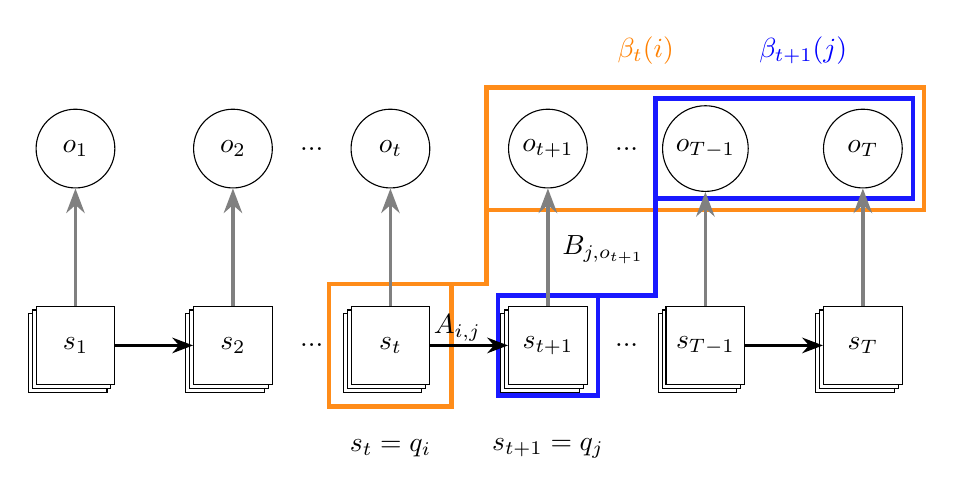
\begin{tikzpicture}[>=Stealth] % 后向算法图示
	\foreach \i/\name in {1/$o_1$,2/$o_2$,3/$o_t$,4/$o_{t+1}$,5/$o_{T-1}$,6/$o_{T}$}{
		\node[circle,draw,text=black,font={\bfseries},minimum size=1cm] 
		(o\i) at (2.0*\i-2.0,2.5){\name};
	}
	
	\foreach \i/\name in {1/$s_1$,2/$s_2$,3/$s_t$,4/$s_{t+1}$,5/$s_{T-1}$,6/$s_{T}$}{
		\node[rectangle,draw,fill=white,text=black,font={\bfseries},minimum size=1cm] 
		(sss\i) at (2.0*\i-2.0-0.1,-0.1){\name};
		\node[rectangle,draw,fill=white,text=black,font={\bfseries},minimum size=1cm] 
		(ss\i) at (2.0*\i-2.0-0.05,-0.05){\name};
		\node[rectangle,draw,fill=white,text=black,font={\bfseries},minimum size=1cm] 
		(s\i) at (2.0*\i-2.0,0){\name};
	}
	
	\draw[outer sep=0.3cm, color=orange!90,line width=1.6pt] ([shift=(45:11mm)] o6.center)--([shift=(135:11mm)] o4.center)--([shift=(225:11mm)] o4.center)--([shift=(135:11mm)] s4.center)--([shift=(45:11mm)] s3.center)--([shift=(315:11mm)] s3.center)--([shift=(225:11mm)] s3.center)--([shift=(135:11mm)]s3.center)--([shift=(135:11mm)]s4.center)--([shift=(225:11mm)]o4.center)--([shift=(315:11mm)]o6.center)--cycle;
	
	\draw[outer sep=0.3cm, color=blue!90,line width=1.6pt] ([shift=(45:9mm)] o6.center)--([shift=(135:9mm)] o5.center)--([shift=(225:9mm)] o5.center)--([shift=(135:9mm)] s5.center)--([shift=(45:9mm)] s4.center)--([shift=(315:9mm)] s4.center)--([shift=(225:9mm)] s4.center)--([shift=(135:9mm)]s4.center)--([shift=(135:9mm)]s5.center)--([shift=(225:9mm)]o5.center)--([shift=(315:9mm)]o6.center)--cycle;
	
	\foreach \i in {1,2,3,4,5,6}{
		\draw[->,color=gray,line width=1.3pt]--(s\i)--(o\i);}
	
	\node[](s0) at (0, 0){};
%	\draw[->,line width=1pt]--(s0)--(s1);
	\draw[->,line width=1pt]--(s1)--(s2);
	\draw[->,line width=1pt]--(s3)--(s4);
	\draw[->,line width=1pt]--(s5)--(s6);
	
%	\node[text = black,scale = 1] at ([shift=(165:20pt)] s1.center) {$\pi(s_{1})$};
	\node[text = black,scale = 1] at ([shift=(60:40pt)] s4.center) {$B_{j,o_{t+1}}$};
	\node[text = black,scale = 1] at ([shift=(15:25pt)] s3.center) {$A_{i,j}$};
	
	\node[text = black,scale = 1] 
	at ([shift=(45:50pt)] o4.center) {$\textcolor{orange}{\beta_{t}(i)}$};
	
	\node[,text = black,scale = 1] 
	at ([shift=(45:50pt)] o5.center) {$\textcolor{blue}{\beta_{t+1}(j)}$};
	
	\foreach \i in {o2,o4, s2, s4}{
		\node[,text = black,scale = 1] 
		at ([shift=(0:10mm)] \i.center) {...}; } % 省略号	
	
	\node[,text = black,scale = 1] 
	at ([shift=(270:8mm)] s3.south) {$s_{t}=q_{i}$}; % 省略号
	
	\node[,text = black,scale = 1] 
	at ([shift=(270:8mm)] s4.south) {$s_{t+1}=q_{j}$}; % 省略号
	
	\label{fig.backward.algo}
\end{tikzpicture}

    后向算法选择把$P(o_{2},...,o_{T}|s_{1}=q_{i})$作为递推终点,记为$\beta_{1}(i)$。那么根据矩阵A和B的定义,$P(O)$如下。
	
	\begin{equation}
		\begin{aligned}
			P(O)
			=&\sum_{i=1}^{N}\pi_{i}B_{i,o_{1}}P(o_{2},...,o_{T}|s_{1}=q_{i}) \\
			=&\sum_{i=1}^{N}\pi_{i}B_{i,o_{1}}\beta_{1}(i) \label{eq.PO.backward.def}
		\end{aligned}
	\end{equation} 
	
 
    由特殊到普遍,$\beta_{t}(i)$为
    \begin{equation}
   		\beta_{t}(i)
   		=\sum_{i=1}^{N}P(o_{t+1},...,o_{T}|s_{t}=q_{i}) \\
    \end{equation} 

    实际上$\beta_{t}(i)$表示的是$t$时刻从状态$q_{i}$出发,观测序列为$(o_{t+1}, ..., o_{T})$的概率。观察图\ref{fig.forward.algo},可以发现相邻时刻的依赖关系。
    
    \begin{equation}
    	\textcolor{orange}{\beta_{t}(i)}
    	=\sum_{j=1}^{N}A_{i,j}B_{j,o_{t}}\textcolor{blue}{\beta_{t+1}(j)} \label{eq.beta.recur}
    \end{equation} 
    
    T时刻本身已经是终点,所以概率$\beta_{T}(i)$为1。
     \begin{equation}
 		\beta_{T}(i)=1 \\
 	\end{equation}    

    从$\beta_{T}$开始往前推,得到$\beta_{1}$,再利用公式\ref{eq.PO.backward.def}求得目标概率。
      
   矩阵形式向我们展示了后向算法为何是后向。
   	\begin{equation}
   		\begin{aligned}
   			\boldsymbol{\beta}&\in \boldsymbol{R}^{n\times T} \\
   			\boldsymbol{\beta}_{:,T}&=\boldsymbol{1} \\
   			\boldsymbol{\beta}_{:,t}&=\boldsymbol{A}(\boldsymbol{\beta}_{:,t+1}\odot  \boldsymbol{B}_{:,o_{t+1}})  \\
   			P(O)&=\pi \bullet (\mathbf{B_{:,o_{1}}} \odot \boldsymbol{\beta}_{:,1})\\
   		\end{aligned}
   	\end{equation}
   
%   	\begin{algorithm}
%   	\caption{Backward Algorithm}
%   	\label{alg:po.backward}
%   	\begin{algorithmic}[1]
%   		\REQUIRE $\pi \in \mathbf{R^{n}},  A \in \mathbf{R^{n\times n}}, B \in \mathbf{R^{n\times m}}, O=(o_{1},o_{2},...,o_{T})$
%   		\ENSURE $P(O) \in (0,1)$
%   		\STATE $\mathbf{\beta_{T}}=\mathbf{1}$
%   		\STATE set $t=T$ 
%   		\WHILE{$t > 1$}
%   		\STATE $\mathbf{\beta_{t}}=\mathbf{A}(\mathbf{\beta_{t+1}}\odot  \mathbf{B_{:,o_{t+1}}})$
%   		\STATE set $t=t-1$
%   		\ENDWHILE
%   		\STATE $P=\mathbf{\pi} \bullet (\mathbf{B_{:,o_{1}}} \odot  \mathbf{\beta_{1}})$
%   		\RETURN $P$
%   	\end{algorithmic}
%   \end{algorithm}
   
\begin{center}
	\fcolorbox{white}{gray!10!cyan!18}{\parbox{.9\linewidth}
		{\rule[0pt]{11cm}{0.07em}\\
			算法: 后向算法(矩阵形式) 
			
			输入:$\pi \in \mathbf{R^{n}},  A \in \mathbf{R^{n\times n}}, B \in \mathbf{R^{n\times m}}, O=(o_{1},o_{2},...,o_{T})$
			
			输出:观测序列$O$的概率$P$
			
			\rule[10pt]{11cm}{0.01em}\\
			1  $\boldsymbol{\beta} = \mathbf{0}^{n\times T}$
			
			2  $\boldsymbol{\beta}_{:,t} =  \boldsymbol{1} $
			
			3  while $t > 1$ do
			
			3  $\qquad \boldsymbol{\beta}_{:,t}=\boldsymbol{A}(\boldsymbol{\beta}_{:,t+1}\odot  \boldsymbol{B}_{:,o_{t+1}})$
			
			4  $\qquad t \leftarrow t-1$
			
			5  end while
			
			6  $P=\pi \bullet (\mathbf{B_{:,o_{1}}} \odot \boldsymbol{\beta}_{:,1})$
			
			7  return $P$
		}
	}
\end{center}

   
   类似的分析可得算法复杂度依然为$O(N^{2}T)$。

\subsubsection{双向算法}
    利用前向概率和后向概率的定义,可以把观测序列的概率写成如下形式。
 	\begin{equation}
 		P(O)= \sum_{i=1}^{N}\alpha_{t}(i)\beta_{t}(i) \label{eq.PO.forward.backward}
 	\end{equation}   
 
    李航《统计学习方法》把概率以下方式展开。
     \begin{equation}
    	P(O)= \sum_{i,j=1}^{M}\alpha_{t}(i)A_{i,j}B_{j,o_{t+1}}\beta_{t+1}(j) \label{eq.PO.forward.backward.lihang}
    \end{equation}

    但这实际上是把$\beta_{t}(i)$按照公式\ref{eq.beta.recur}展开而已,显得稍微繁冗。因此我们采用公式\ref{eq.PO.forward.backward}即可。
    由于本文讨论的是一阶马尔科夫链,因此序列$o_{1},...,o_{t}$与$o_{t+1},...,o_{T}$仅仅通过$s_{t}$这一时刻状态关联起来。如果$s_{t}$给定,那么
    $P(o_{1},...,o_{t},s_{t}=q_{i})$与$P(o_{t+1},...,o_{T},s_{t}=q_{i})$是独立的。参照下图。
    
    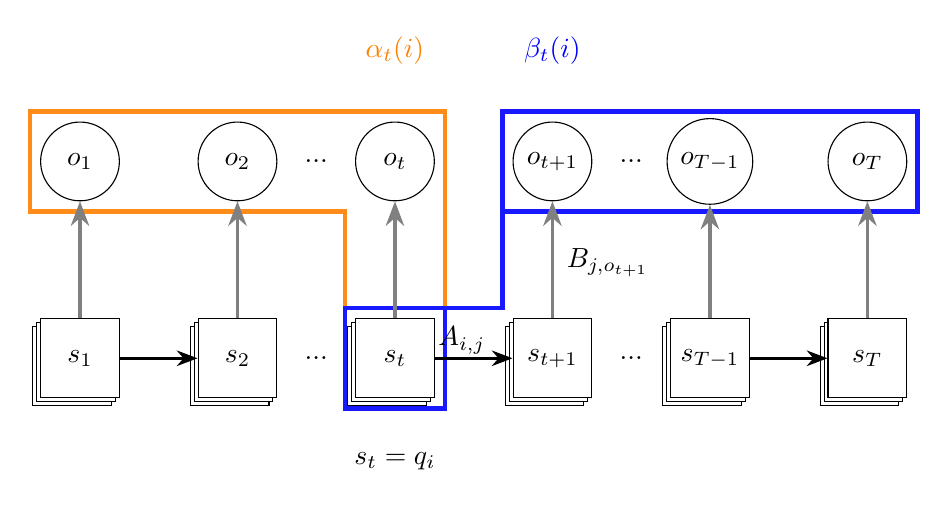
\begin{tikzpicture}[>=Stealth] % 前向后向算法图示
    	\foreach \i/\name in {1/$o_1$,2/$o_2$,3/$o_t$,4/$o_{t+1}$,5/$o_{T-1}$,6/$o_{T}$}{
    		\node[circle,draw,text=black,font={\bfseries},minimum size=1cm] 
    		(o\i) at (2.0*\i-2.0,2.5){\name};
    	}
    	
    	\foreach \i/\name in {1/$s_1$,2/$s_2$,3/$s_t$,4/$s_{t+1}$,5/$s_{T-1}$,6/$s_{T}$}{
    		\node[rectangle,draw,fill=white,text=black,font={\bfseries},minimum size=1cm] 
    		(sss\i) at (2.0*\i-2.0-0.1,-0.1){\name};
    		\node[rectangle,draw,fill=white,text=black,font={\bfseries},minimum size=1cm] 
    		(ss\i) at (2.0*\i-2.0-0.05,-0.05){\name};
    		\node[rectangle,draw,fill=white,text=black,font={\bfseries},minimum size=1cm] 
    		(s\i) at (2.0*\i-2.0,0){\name};
    	}
    	
		\draw[outer sep=0.3cm, color=orange!90,line width=1.6pt] ([shift=(135:9mm)] o1.center)--([shift=(45:9mm)] o3.center)--([shift=(315:9mm)]s3.center)--([shift=(225:9mm)] s3.center)--([shift=(225:9mm)] o3.center)--([shift=(225:9mm)]o1.center)--cycle;
    	
		\draw[outer sep=0.3cm, color=blue!90,line width=1.6pt] ([shift=(45:9mm)] o6.center)--([shift=(135:9mm)] o4.center)--([shift=(225:9mm)] o4.center)--([shift=(135:9mm)] s4.center)--([shift=(45:9mm)] s3.center)--([shift=(315:9mm)] s3.center)--([shift=(225:9mm)] s3.center)--([shift=(135:9mm)]s3.center)--([shift=(135:9mm)]s4.center)--([shift=(225:9mm)]o4.center)--([shift=(315:9mm)]o6.center)--cycle;
    	
    	\foreach \i in {1,2,3,4,5,6}{
    		\draw[->,color=gray,line width=1.3pt]--(s\i)--(o\i);}
    	
    	\node[](s0) at (0, 0){};
    	%	\draw[->,line width=1pt]--(s0)--(s1);
    	\draw[->,line width=1pt]--(s1)--(s2);
    	\draw[->,line width=1pt]--(s3)--(s4);
    	\draw[->,line width=1pt]--(s5)--(s6);
    	
    	%	\node[text = black,scale = 1] at ([shift=(165:20pt)] s1.center) {$\pi(s_{1})$};
    	\node[text = black,scale = 1] at ([shift=(60:40pt)] s4.center) {$B_{j,o_{t+1}}$};
    	\node[text = black,scale = 1] at ([shift=(15:25pt)] s3.center) {$A_{i,j}$};
    	
    	\node[text = black,scale = 1] 
    	at ([shift=(90:40pt)] o3.center) {$\textcolor{orange}{\alpha_{t}(i)}$};
    	
    	\node[,text = black,scale = 1] 
    	at ([shift=(90:40pt)] o4.center) {$\textcolor{blue}{\beta_{t}(i)}$};
    	
    	\foreach \i in {o2,o4, s2, s4}{
    		\node[,text = black,scale = 1] 
    		at ([shift=(0:10mm)] \i.center) {...}; } % 省略号	
    	
    	\node[,text = black,scale = 1] 
    	at ([shift=(270:8mm)] s3.south) {$s_{t}=q_{i}$}; % 省略号
    	
    	\label{fig.forward.backward.algo}
    \end{tikzpicture}
    
%    矩阵形式由前文可以简单得到。
%    
%       \begin{equation}
%    	\begin{aligned}
%    		\boldsymbol{\alpha} &\in \mathbf{R}^{n\times T}, \boldsymbol{\beta} \in \mathbf{R}^{n\times T}\\
%    		\boldsymbol{\alpha}_{:,1}&=\pi \odot  \boldsymbol{B}_{:, o_{1}} \\
%    		\boldsymbol{\alpha}_{:,t+1}&=(\boldsymbol{A^{T}}\boldsymbol{\alpha}_{:,t})\odot  \boldsymbol{B}_{:, o_{t+1}}\\
% 			\boldsymbol{\beta}_{:,T}&=\boldsymbol{1}\\
% 			\boldsymbol{\beta}_{:,t}&=\boldsymbol{A}(\boldsymbol{\beta}_{:,t+1}\odot  \boldsymbol{B}_{:,o_{t+1}}) \\
% 			P(O)&=\pi \bullet (\mathbf{B_{:,o_{1}}} \odot \boldsymbol{\beta}_{:,1})
% 	\end{aligned}
% \end{equation}


\begin{center}
	\fcolorbox{white}{gray!10!cyan!18}{\parbox{.9\linewidth}
		{\rule[0pt]{11cm}{0.07em}\\
			算法: 双向算法(矩阵形式) 
			
			输入:$\pi \in \mathbf{R^{n}},  A \in \mathbf{R^{n\times n}}, B \in \mathbf{R^{n\times m}}, O=(o_{1},o_{2},...,o_{T})$
			
			输出:观测序列$O$的概率$P$,各个时刻的前向概率矩阵$\boldsymbol{\alpha}$和后向矩阵$\boldsymbol{\beta}$
			
			\rule[10pt]{11cm}{0.01em}\\
			1  $\boldsymbol{\alpha} = \mathbf{0}^{n\times T}, \boldsymbol{\beta} = \mathbf{0}^{n\times T}$
			
			2  $\boldsymbol{\beta}_{:,T} =  \boldsymbol{1} $
			
			3  while $t > 1$ do
			
			4  $\qquad \boldsymbol{\beta}_{:,t}=\boldsymbol{A}(\boldsymbol{\beta}_{:,t+1}\odot  \boldsymbol{B}_{:,o_{t+1}})$
			
			5  $\qquad t \leftarrow t-1$
			
			6  end while

            7  $\boldsymbol{\alpha}_{:,1}=\pi \odot  \boldsymbol{B}_{:, o_{1}} $
            
		    8  while $t < T$ do

			9  $\qquad \boldsymbol{\alpha}_{:,t+1}=(\boldsymbol{A^{T}}\boldsymbol{\alpha}_{:,t})\odot  \boldsymbol{B}_{:, o_{t+1}}$

			10  $\qquad t \leftarrow t+1$

			11  end while
			
			12  $d=(\boldsymbol{\alpha} \odot \boldsymbol{\beta})_{:,T/2}$
			
			13  $P=d/||d||$
			
			14  return $P,\boldsymbol{\alpha},\boldsymbol{\beta}$
		}
	}
\end{center}
    
    从现在起,前向概率和后向概率分别用$\boldsymbol{\alpha}$和$\boldsymbol{\beta}$的矩阵元来表示。
    
    \begin{equation}
    	\begin{aligned}
    		\alpha_{t}(i)&=\boldsymbol{\alpha}_{i,t} = P(o_1,o_2,...,o_t, s_t=q_i)\\
    		\beta_{t}(i)&=\boldsymbol{\beta}_{i,t} = P(o_{t+1},...,o_T, s_t=q_i)
    	\end{aligned}
    \end{equation}
%\begin{algorithm}
%	\caption{Bidirection Algorithm}
%	\label{alg:po.bidirec}
%	\begin{algorithmic}[1]
%		\REQUIRE $\pi \in \mathbf{R^{n}}, \mathbf{ A} \in \mathbf{R^{n\times n}}, \mathbf{B} \in \mathbf{R^{n\times m}}, O=(o_{1},o_{2},...,o_{T})$
%		\ENSURE $P \in (0,1), \boldsymbol{\alpha} \in \mathbf{R^{n \times T}}, \boldsymbol{\beta} \in \mathbf{R^{n \times T}}$
%		\STATE set $t=1, \mathbf{\alpha}=\mathbf{0}, \mathbf{\beta}=\mathbf{0}$ 
%		\STATE $\boldsymbol{\alpha}_{:,t}=\mathbf{\pi}\odot  \boldsymbol{B}_{:, o_{1}}$ 
%		\WHILE{$t < T$}
%		\STATE $\boldsymbol{\alpha}_{:,t+1} = (\mathbf{A}^{T}\mathbf{\boldsymbol{\alpha}}_{:, t})\odot  \mathbf{B}_{:, o_{t+1}}$
%		\STATE set $t=t+1$
%		\ENDWHILE
%		\STATE set $t=T$
%		\STATE $\boldsymbol{\beta}_{:,T}=\mathbf{1}$
%		\WHILE{$t > 1$}
%		\STATE $\boldsymbol{\beta}_{:,t}=\mathbf{A}(\boldsymbol{\beta}_{:,t+1}\odot  \mathbf{B}_{:,o_{t+1}})$
%		\STATE set $t=t-1$
%		\ENDWHILE
%		\STATE select $t^{*} = int(T/2)$
%		\STATE $P=\boldsymbol{\alpha}_{:,t^{*}} \bullet \boldsymbol{\beta}_{:,t^{*}} $
%		\RETURN $P, \boldsymbol{\alpha}, \boldsymbol{\beta} $
%	\end{algorithmic}
%\end{algorithm}



 
\subsubsection{若干概率和期望值}
	
	利用序列$O$概率的计算产物,可以得到一些有用的概率和期望值。
	
	1. 给定模型$h$和观测序列$O$,时刻$t$状态为$q_{i}$的概率。

    类似地,我们也使用$\boldsymbol{\gamma}$的矩阵元$\boldsymbol{\gamma}_{i,t}$来表示给定时刻$t$状态为$q_{i}$的概率。
   
   	\begin{equation}
   	\boldsymbol{\gamma}_{i,t}= P(s_{t}=q_{i}|o_{1},...,o_{T})
   \end{equation}
    
	参照前文的前向后向算法以及示意图,轻易得到$\gamma_{t}(i)$。
	\begin{equation}
		\begin{aligned}
			\boldsymbol{\gamma}_{i,t}&= \frac{\boldsymbol{\alpha}_{i,t}\boldsymbol{\beta}_{i,t}}{P(O)} \\
			&= \frac{\boldsymbol{\alpha}_{i,t}\boldsymbol{\beta}_{i,t}}{\sum_{i=1}^{N}\boldsymbol{\alpha}_{i,t}\boldsymbol{\beta}_{i,t}}
		\end{aligned}
	\end{equation}

    写成矩阵形式。
    \begin{equation}
    	\begin{aligned}
    		\boldsymbol{\gamma}&= \frac{\boldsymbol{\alpha}\odot \boldsymbol{\beta}}{P(O)} \\
    		P(O)&=  \boldsymbol{1}\bullet(\boldsymbol{\alpha}\odot \boldsymbol{\beta})_{:,T/2}
    	\end{aligned}
    \end{equation}
    
	2. 给定模型$h$和观测序列$O$,时刻$t$状态为$q_{i}$且时刻$t+1$状态为$q_{j}$的概率。
	
	类似地,我们用三阶矩阵$\boldsymbol{\gamma}$的矩阵元$\boldsymbol{\gamma}_{t,i,j}$表示这一概率。
	\begin{equation}
		\boldsymbol{\xi}_{t,i,j}= P(s_{t}=q_{i},s_{t+1}=q_{j}|o_{1},...,o_{T})
	\end{equation}   
	参照前文的双算法\ref{eq.PO.forward.backward.lihang},轻易得到$\boldsymbol{\xi}_{t,i,j}$。
	
	\begin{equation}
		\begin{aligned}
			\boldsymbol{\xi}_{t,i,j}&= \frac{\boldsymbol{\alpha}_{i,t}\boldsymbol{A}_{i,j}\boldsymbol{B}_{j,o_{t+1}}\boldsymbol{\beta}_{j,t+1}}{P(O)} 
		\end{aligned}
	\end{equation}

   写成矩阵形式。

	\begin{equation}
	\begin{aligned}
		\boldsymbol{\xi}_{t,:,:}&=\frac{
		\boldsymbol{A} \odot (\boldsymbol{\alpha}_{:,t} \otimes (\boldsymbol{B}_{:,o_{t+1}} \odot \boldsymbol{\beta}_{:,t+1}))}{P(O)}, t=1,2,...,T-1
		 %\frac{\boldsymbol{\alpha}_{i,t}\boldsymbol{A}_{i,j}\boldsymbol{B}_{j,o_{t+1}}\boldsymbol{\beta}_{j,t+1}}{P(O)} 
	\end{aligned}
\end{equation}   
   

   3. 给定观测O状态$q_{i}$出现次数的期望值为$\sum_{t=1}^{T}\boldsymbol{\gamma}_{i,t}$。

   4. 给定观测O状态$q_{i}$转移到$q_{j}$次数的期望值为$\sum_{t=1}^{T-1}\boldsymbol{\xi}_{t,i,j}$。


\subsection{HMM的参数估计}
    隐马尔科夫模型的学习,如果训练数据同时包含观测序列和对应的状态序列,那么可以由监督学习实现;如果仅包含观测序列,则依靠无监督学习。后者可以依靠Baum-Welch算法,实际上该算法是EM算法在HMM的特化。
\subsubsection{HMM的有监督学习:给定状态序列、观测序列估计参数}
    如果训练数据包含$n$个长度相同的观测序列和对应的状态序列$\{(O_{1},S_{1}),\\(O_{2},S_{2}),...,(O_{n},S_{n})\}$,那么利用极大似然来估计参数即可。
    
    1. 估计初始状态概率$\pi$
    把样本中初始时刻为状态$q_{i}$的频数除以所有频数之和即可。
    
        \begin{equation}
    	\pi_{i}=\frac{n_{s_{1}=q_{i}}}{\sum_{i}n_{s_{1}=q_{i}}}
    \end{equation} 
    
    2. 估计转移概率$A_{i,j}$
    把样本中t时刻从状态$q_{i}$转移到t+1时刻$q_{j}$的频数记为$\widetilde{A}_{i,j}$,则转移矩阵$A$的矩阵元$A_{i,j}$如下。
    \begin{equation}
    	A_{i,j}=\frac{\widetilde{A}_{i,j}}{\sum_{i,j}\widetilde{A}_{i,j}}
    \end{equation} 
    
    3. 估计观测概率$B_{j,k}$
    把样本中t时刻状态为$q_{j}$,观测$o_{t}=v_{k}$的次数记为$\widetilde{B}_{j,k}$,则观测矩阵$B$的矩阵元$B_{j,k}$如下。
    \begin{equation}
		B_{j,k}=\frac{\widetilde{B}_{j,k}}{\sum_{k}\widetilde{B}_{j,k}}
	\end{equation} 
   
    
\subsubsection{HMM的无监督学习:仅从观测序列估计参数}
	训练数据包含$n$个长度相同的观测序列$\{O_{1},O_{2},...,O_{n}\}$,以及隐藏状态集合$Q$的元素个数,目标是学习HMM的参数
	$h=(A,B,\pi)$。显然隐藏状态序列是隐变量,HMM是含有隐变量的概率模型,其参数学习可以用EM来实现。
	
	\begin{equation}
		P(O|h)=\sum_{S}P(O|S,h)P(S|h)
	\end{equation} 

    我们先来简短回顾一下EM算法。EM算法核心是对Q函数的极大化。Q函数的意义是先用上轮参数条件、已有数据算出隐变量的分布,再求
    当前轮次的参数条件下的完全数据的概率对数在隐变量分布下的期望。说白了其实就是完全数据在隐变量分布下的“似然”期望值,Q函数越大,说明新参数下的模型与数据“相似”程度进步越大。$Y,Z,\theta$分别为观测变量,隐变量,模型参数,$\theta^{(i)}$是上轮模型参数。
    \begin{equation}
    	\begin{aligned}
    		Q(\theta, \theta^{(i)})=\sum_{Z}P(Z|Y,\theta^{(i)})\log{P(Y,Z|\theta)}
    	\end{aligned}
    \end{equation}
    如果我们给该函数乘以一个常数项$P(Y|\theta^{(i)})$,那么Q函数的“似然”的本质就更容易理解了。显然该常数不影响新参数$\theta$
    的估计。
    
    \begin{equation}
    	\begin{aligned}
    		Q(\theta, \theta^{(i)})P(Y|\theta^{(i)})&=P(Y|\theta^{(i)})\sum_{Z}\frac{P(Y,Z|\theta^{(i)})}{P(Y|\theta^{(i)})}\log{P(Y,Z|\theta)}\\
    		&=\sum_{Z}P(Y,Z|\theta^{(i)})\log{P(Y,Z|\theta)}
    	\end{aligned}
    \end{equation}
    

    回到HMM,我们先确定完全数据的对数似然,即所谓的E步。$P(O,S|\widetilde{h})$是根据老参数估计的完全数据的概率。
	\begin{equation}
		\begin{aligned}
			Q(h,\widetilde{h})
			&=\sum_{S}P(O,S|\widetilde{h})\log{P(O,S|h)}\\
		\end{aligned}
	\end{equation}
    
    结合HMM,完全数据概率如下(分配-呈现-转换-呈现-...转换-呈现)。
	\begin{equation}
	\begin{aligned}
		P(O,S|h)=\pi_{s_{1}}B_{s_{1},o_{1}}A_{s_{1},s_{2}}B_{s_{2},o_{2}}...A_{s_{T-1}s_{T}}B_{s_{T},o_{T}}\\
	\end{aligned}
	\end{equation}

    于是,完全数据的对数似然可以写成
   	\begin{equation}\label{eq.log.likelihood}
   	\begin{aligned}
   		\log{Q(h,\widetilde{h})}=&\textcolor{red}{\sum_{S}P(O,S|\widetilde{h})\log{\pi_{s_{1}}}}+\\
   		                         &\textcolor{blue}{\sum_{S}P(O,S|\widetilde{h})\sum_{t=1}^{t=T-1}\log{A_{s_{t},s_{t+1}}}}+\\
   		                         &\textcolor{teal}{\sum_{S}P(O,S|\widetilde{h})\sum_{t=1}^{t=T}\log{B_{s_{t},o_{t}}}}    
   	\end{aligned}
   \end{equation}  
   
    我们注意到,上式右边三项分别只和与$\pi,A,B$有关,那么在对完全数据极大化估计$h=(\pi, A, B)$时,可以分项独立进行。但是,上式是对所有可能存在的长度为T的状态序列进行求和,序列的个数等于状态数的序列长度次方$N^T$,计算复杂度过高,我们需要分别转换一下。
   
    例如对于式\ref{eq.log.likelihood}右边第一项,可以作如下处理。
    \begin{equation}
   	\begin{aligned}
   		\textcolor{red}{\sum_{S}P(O,S|\widetilde{h})\log{\pi_{s_{1}}}}=\sum_{i}P(O,s_{1}=q_{i}|\widetilde{h})\log{\pi_{i}}\\
   	\end{aligned}
   \end{equation}  
    
    这是因为$P(O,S|\widetilde{h})$是对序列$S$求和,但$S$中与$\pi_{s_{1}}$有关的仅仅是$s_{1}$而已,那么改成针对$s_{1}$的所有可能取值$q_{i}$即可达到同样的目的。
   
    同理,式\ref{eq.log.likelihood}右边第二项针对$S$和$t$求和,与$S$有关的仅有$s_t$与$s_{t+1}$两项,因此改成如下形式。
    \begin{equation}
   	\begin{aligned}
   		\textcolor{blue}{\sum_{S}P(O,S|\widetilde{h})\sum_{t=1}^{t=T-1}\log{A_{s_{t},s_{t+1}}}}=\sum_{i=1}^{i=N}\sum_{j=1}^{j=N}\sum_{t=1}^{t=T-1}P(O,s_t=q_i, s_{t+1}=q_j|\widetilde{h})\log{A_{i,j}}\\
   	\end{aligned}
   \end{equation}  
   
    式\ref{eq.log.likelihood}右边第三项针对$S$和$t$求和,与$S$有关的仅有$s_t$一项,改成针对$s_{t}$的所有可能取值求和。但给定观测序列$O$后$o_{t}$已全部确定,那么改成如下形式。

    \begin{equation}
	\begin{aligned}
		\textcolor{teal}{\sum_{S}P(O,S|\widetilde{h})\sum_{t=1}^{t=T}\log{B_{s_{t},o_{t}}}}=\sum_{i=1}^{i=N}\sum_{j=1}^{j=M}\sum_{t=1}^{t=T-1}P(O,s_t=q_i|\widetilde{h})I(o_t=v_j)\log{B_{i,j}}\\
	\end{aligned}
	\end{equation}    
   
    以下我们可以开展EM算法的M步了,即完全数据的对数似然针对模型参数进行极大化。
   
    针对第一项,注意到$\pi_{i}$满足约束条件$\sum_{i}\pi_{i}$,利用拉格朗日乘子法,写出拉格朗日函数。
   
   \begin{equation}
   	\sum_{i}^{N}P(O,s_{1}=q_{i}|\widetilde{h})\log{\pi_{i}}+\lambda(\sum_{i}\pi_{i}-1)
   \end{equation}
   
    对$\pi_{i}$求导使其导数为0。
   \begin{equation}
   	P(O,s_{1}=q_{i}|\widetilde{h})+\lambda\pi_{i}=0 \label{eq.pi.lagrange}
   \end{equation}
   
    对$i$求和之后得到$\lambda$如下。
   \begin{equation}
   	\lambda=-P(O|\widetilde{h})
   \end{equation}

    代入式\ref{eq.pi.lagrange},得到$\pi_{i}$。
    \begin{equation}
    	\begin{aligned}
    		\pi_{i}&=\frac{P(O,s_1=q_i|\widetilde{h})}{P(O|\widetilde{h})}\\
    		&=\boldsymbol{\gamma}_{i,t}
    	\end{aligned}
    \end{equation}
  
  同样方式处理第二项,约束条件为$\sum_{j=1}^{N}A_{i,j}=1$,利用拉格朗日乘子法写出函数并对$A_{i,j}$求导,使其为0。
  类似可得$A_{i,j}$。其实这里根据i=1,2,...,N进行了N次操作。
   
  \begin{equation}
  	\begin{aligned}
  		A_{i,j}=&\frac{\sum_{t=1}^{t=T-1}P(O,s_t=q_i, s_{t+1}=q_j|\widetilde{h})}{\sum_{t=1}^{t=T}P(O,s_t=q_i|\widetilde{h})}\\
  		=&\frac{\sum_{t=1}^{t=T-1}\boldsymbol{\xi}_{t,i,j}}{\sum_{t=1}^{t=T}\boldsymbol{\gamma}_{i,t}}
  	\end{aligned}
  \end{equation}

  处理第三项时,约束条件为$\sum_{j=1}^{M}B_{i,j}=1$,类似操作可得$B_{i,j}$。由于约束条件有M个,同样进行了M次操作。
  \begin{equation}
  	\begin{aligned}
  	B_{i,j}&=\frac{\sum_{t=1}^{t=T-1}P(O,s_t=q_i|\widetilde{h})I(o_t=v_j)}{\sum_{t=1}^{t=T-1}P(O,s_t=q_i|\widetilde{h})}\\
  	&=\frac{\sum_{t=1}^{t=T}\boldsymbol{\gamma}_{i,t}I(o_t=v_j)}{\sum_{t=1}^{t=T}\boldsymbol{\gamma}_{i,t}}
  	\end{aligned}
  \end{equation}
  
  我们注意到,以上结果都可以利用双向算法的副产物的副产物$\boldsymbol{\gamma}$和$\boldsymbol{\xi}$来表示。
  
  \clearpage
  
  \rule[0pt]{12cm}{0.1em}
  
  算法 \quad Baun-Welch算法
  
  \rule[5pt]{12cm}{0.05em}
  
  输入:观测序列 $O=(o_1, o_2,..., o_T)$,初始HMM模型$h^{(0)}=(\pi^{(0)}, \boldsymbol{A^{(0)}}, \boldsymbol{B^{(0)}})$
    
  输出:HMM参数 $h=(\pi, \boldsymbol{A}, \boldsymbol{B})$
  
  \rule[10pt]{12cm}{0.05em}
  
  (1) 对于$i=0$,把$O$与$h^{(0)}$输入双向模型,得到$P, \boldsymbol{\alpha^{(0)}}, \boldsymbol{\beta^{(0)}}$  
  
  (2) 递推。对于$i=1,2,...$,
  
  \begin{equation}
  	\begin{aligned}
  		&\boldsymbol{\gamma}=\boldsymbol{\alpha^{(i)}}\odot \boldsymbol{\beta^{(i)}}\\
  		&\boldsymbol{\gamma}_{:,t}=\boldsymbol{\gamma}_{:,t} / ||\boldsymbol{\gamma}_{:,t}||,t=1,2,...,T \\
  	\end{aligned}  	
  \end{equation}
  

\subsection{预测状态序列}
  
  \subsubsection{近似算法}
    近似算法的思路是在每个时刻t选择在该时刻出现概率最高的状态$s_{t}^{*}$,得到状态序列$S^{*}=(s_{1}^{*},s_{2}^{*},...,s_{T}^{*})$,并作为预测的结果。

    给定HMM模型$h=(\pi, \boldsymbol{A}, \boldsymbol{B})$和观测序列O,在时刻t处于状态$q_i$的概率是$\boldsymbol{\gamma}_{i,t}$。
    
    \begin{equation}
    	\begin{aligned}
    		\gamma_{i,t}=\frac{\boldsymbol{\alpha}_{i,t}\boldsymbol{\beta}_{i,t}}{P(O)}\\
    	\end{aligned}
    \end{equation}

    在每一时刻$t$,最有可能的状态$i^{*}=argmax_{1\le i \le N}\boldsymbol{\gamma}_{i,t},\quad t=1,2,...,T$。从而得到序列$S^{*}=(s_{1}^{*},s_{2}^{*},...,s_{T}^{*})$。
  
    近似算法虽然计算简单,但是每个节点局部最优不保证整体最优,因为这样预测出的状态序列中可能存在转移概率为0的相邻状态。
    
  \subsubsection{Viterbi算法} 
    Viterbi算法
    $\Phi$
    
\end{document}
